\documentclass{article}

\usepackage{mystyle}
\usepackage{myvars}

%-----------------------------

\begin{document}

  \maketitle

  \part{Ejercicios Montgomery:}

  \setcounter{section}{2}
  \subsection{En la tabla B.1 del apéndice aparecen datos sobre el desempeño de los 26 equipos de la Liga Nacional de Fútbol en 1976. Se cree que la cantidad de yardas ganadas por tierra por los contrarios ($x_8$) tiene un efecto sobre la cantidad de juegos que gana un equipo ($y$).}
  \subsubsection{Ajustar un modelo de regresión lineal simple que relacione los juegos ganados, $y$, con las yardas ganadas por tierra por los contrarios, $x_8$.}

  \begin{equation}
  \label{eq:simple-linear-regression-model}
    y_i = \beta_0 + \beta_1x_8_i + \varepsilon_i
  \end{equation}
  \paragraph{}
  Analizaremos el modelo de la ecuación \ref{eq:simple-linear-regression-model} mediante un estudio de regresión lineal simple, con $y$ como variable dependiente, $x_8$ como variable independiente, $\beta_0$ el intercepto, y $\beta_1$ la pendiente. $\varepsilon$ es el error aleatorio.

  \paragraph{}
  El procedimiento \textit{REG} permite estimar los valores del intercepto y la pendiente, y analizar las hipótesis nulas:

    \begin{align}
      H_0: \beta_0 = 0\\
      H_0': \beta_1 = 0
      \label{mont:hipotesisnulas}
    \end{align}

  \paragraph{}
  La hipótesis más importante en la regresión es la que incumbe a $\beta_1$, ya que si la pendiente de la recta es 0, no existe regresión, y se trata de una población simple sobre la que $x_8$ no tiene efecto.

  \begin{figure}[H]
    \centering
    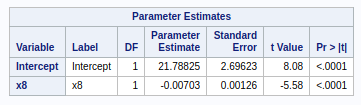
\includegraphics[width=.5\textwidth]{img/montgomery/procreg.png}
    \caption{Estimadores y p-valores para la regresión.}
    \label{img:mont-procreg}
  \end{figure}

  \paragraph{}
  Como podemos ver, el \textit{p-valor} para $\beta_1$ está por debajo de $0,05$, por lo que podemos rechazar la hipótesis nula con una confianza del 95\%. El \textit{p-valor} para el intercepto también permite rechazar la hipótesis nula.

  \paragraph{}
  Por tanto, los estimadores son:

  \begin{align}
    \hat\beta_0 = 21.78825\\
    \hat\beta_1 = -0.00703
  \end{align}

  \paragraph{}
  Con la recta de regresión:

  \begin{equation}
    y_i = 21.78825 -0.00703x_8_i + \varepsilon_i
  \end{equation}

  \paragraph{}
  La interpretación de estos parámetros es que con 0 yardas ganadas por el contrario, un equipo gana de media $21,78825$ juegos, y que por cada yarda que gana el contrario, el equipo pierde de media $0.00703$ juegos.

  \begin{figure}[H]
    \centering
    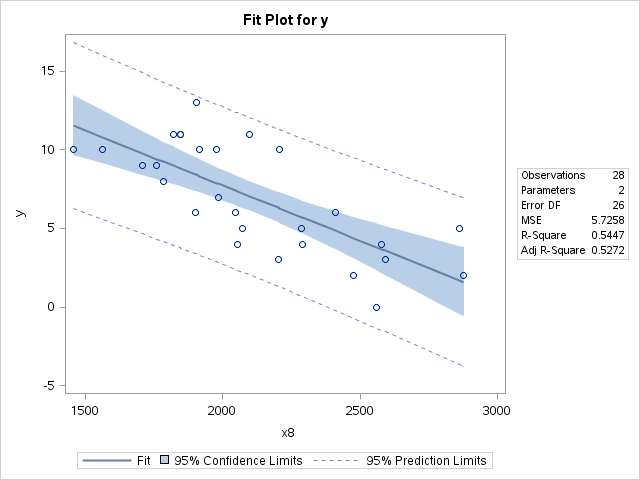
\includegraphics[width=.8\linewidth]{img/montgomery/fitplot.png}
    \caption{Fit plot del modelo de regresión lineal simple}
    \label{img:mont-fitplot}
  \end{figure}

  \subsubsection{Formar la tabla de análisis de varianza y probar el significado de la regresión.}

  \paragraph{}
  La tabla de análisis de la varianza se obtiene también mediante el procedimiento \textit{REG}.

  \begin{figure}[H]
    \centering
    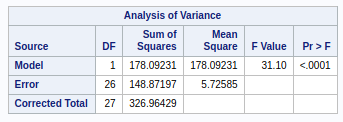
\includegraphics[width=.5\linewidth]{img/montgomery/anovatable.png}
    \caption{Tabla de análisis de la varianza}
    \label{img:mont-anova}
  \end{figure}

  \paragraph{}
  Esta tabla nos permite obtener la suma de cuadrados del modelo y del error, lo cual nos da un modo alternativo de hacer el contraste sobre el coeficiente $\beta_1$. \textit{Mean Square} para el \textit{Error} es el estimador de la varianza $\sigma^2$ obtenida por el error aleatorio $\varepsilon$. Si se cumple la hipótesis $H_0: \beta_1=0$, \textit{Mean Square} para el \textit{Model} también es un estimador de la varianza $\sigma^2$. Por tanto

  \begin{equation}
    F = \frac{MSM}{MSE}
  \end{equation}

  \paragraph{}
  es un estadístico que permite realizar el test de hipótesis sobre la hipótesis nula $H_0$. Esta tabla también nos proporciona el \textit{p-valor} para este contraste, que es menor que $0,05$, por lo que podemos rechazar la hipótesis, y afirmar que existe regresión con un 95\% de confianza.

  \subsubsection{Determinar un intervalo de confianza de 95\% para la pendiente.}

  \paragraph{}
  La pendiente es el parámetro $\beta_1$, y podemos obtener los intervalos de confianza para los parámetros mediante el procedimiento \textit{REG}, añadiendo la opción \textit{CLB} al modelo.

  \begin{figure}[H]
    \centering
    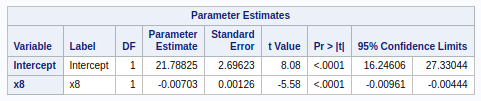
\includegraphics[width=.6\linewidth]{img/montgomery/icestim.png}
    \caption{Estimadores para los parámetros con intervalos de confianza del 95\%}
  \end{figure}

  \paragraph{}
  El intervalo de confianza de la pendiente es el correspondiente al parámetro $x_8$, por lo que la pendiente se situa entre $-0.00961$ y $-0.00444$.

  \subsubsection{¿Qué porcentaje de variabilidad total da $y$, y explica este modelo?}

  \paragraph{}
  Para obtener la medida de variabilidad total de $y$ debemos volver a la tabla de análisis de varianza del apartado \textbf{b}:

  \begin{figure}[H]
    \centering
    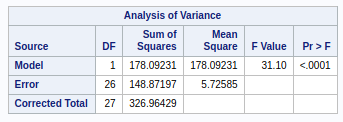
\includegraphics[width=.5\linewidth]{img/montgomery/anovatable.png}
    \caption{Tabla de análisis de la varianza}
    \label{img:mont-anova}
  \end{figure}

  \paragraph{}
  Esta tabla nos da la \textit{Suma de cuadrados total}, que en este caso es igual a $326,96429$. Para obtener la variabilidad de la muestra, conocida como $MST$, se divide este valor por sus grados de libertad, que son $N-1$, siendo $N$ el número de observaciones.

  \begin{equation}
    MST = \frac{SST}{N-1} = \frac{326,96429}{27} = 12.109788519
  \end{equation}

  \paragraph{}
  Este valor $MST$ es la variabilidad total de la muestra $\sigma_T^2$, parte de la cual intentamos explicar mediante el modelo de regresión lineal simple. Existirá otra parte explicada por el error aleatorio, $\sigma^2$.

  \paragraph{}
  Para calcular la cantidad de variabilidad que explica el modelo podemos calcular:

  \begin{equation}
    \frac{SS_{Modelo}}{SS_{Total}}
  \end{equation}

  \paragraph{}
  Que es un coeficiente conocido como $R^2$, que también podemos obtener directamente con la siguiente tabla obtenida del procedimiento \textit{REG}:

  \begin{figure}[H]
    \centering
    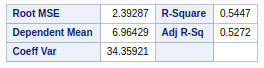
\includegraphics[width=.35\linewidth]{img/montgomery/tablaregaux.png}
    \caption{Coeficientes de la Regresión Lineal Simple.}
    \label{img:mont-tabla-aux}
  \end{figure}

  \paragraph{}
  \textit{R-square} indica que el modelo de regresión explica un $54.47\%$ de la variabilidad. También puede interpretarse como un indicador de cómo de bien se ajustan los datos a la línea de regresión ajustada.


  \subsubsection{Determinar un intervalo de confianza de 95\% para la cantidad promedio de juegos ganados, si la distancia ganada por tierra por los contrarios se limita a 2000 yardas.}

  \subsection{Supóngase que se quiere usar el modelo desarrollado en el problema 2.1 para pronosticar la cantidad de juegos que ganará un equipo si puede limitar los avances por tierra de sus contrarios a 1800 yardas. Determinar un estimado de punto de la cantidad de juegos ganados cuando $x_8=1800$. Determinar un intervalo de predicción de 90\% para la cantidad de juegos ganados.}

  \part{Código Fuente}


\end{document}
